% !TEX encoding = UTF-8 Unicode

\documentclass[a4paper]{article}

\usepackage{color}
\usepackage{url}
\usepackage[T2A]{fontenc} % enable Cyrillic fonts
\usepackage[utf8]{inputenc} % make weird characters work
\usepackage{graphicx}
\usepackage{amsmath}
\usepackage{amssymb}
\usepackage{amsthm}
\usepackage{listings}
\usepackage{verbatim}

\lstdefinestyle{stil} {
	numberstyle=\tiny\color[rgb]{0.6, 0.6, 0.6},
	numbers=left
}


\lstset{style=stil}

\usepackage[english,serbian]{babel}

\usepackage[unicode]{hyperref}
\hypersetup{colorlinks,citecolor=green,filecolor=green,linkcolor=blue,urlcolor=blue}

\newtheorem{primer}{Primer}[section]
\newtheorem{definicija}{Definicija}
\newtheorem{teorema}{Teorema}

\usepackage{mathptmx}

\usepackage{graphicx}
\makeatletter
\providecommand{\bigsqcap}{%
  \mathop{%
    \mathpalette\@updown\bigsqcup
  }%
}
\newcommand*{\@updown}[2]{%
  \rotatebox[origin=c]{180}{$\m@th#1#2$}%
}
\makeatother

\begin{document}

\title{Apstraktna interpretacija\\ \small{Seminarski rad u okviru kursa\\Metodologija stručnog i naučnog rada\\ Matematički fakultet}}

\author{Ozren Demonja, Stefan Maksimović, Marko Crnobrnja\\ mi12319@alas.matf.bg.ac.rs, mi12078@alas.matf.bg.ac.rs, mi12024@alas.matf.bg.ac.rs}
\date{1.~april 2017.}
\maketitle

\abstract{U ovom tekstu predstavljena je metoda apstraktne interpretacije, objašnjeni uslovi njenog nastajanja i navedene njene primene u savremenom računarstvu za optimizaciju i verifikaciju softvera. Radi objašnjenja apstraktne interpretacije naveden je jedan neformalan neprogramski primer kao i celo poglavlje u kome je detaljno razmotren primer jednog C++ koda. Na kraju je data i matematička formalizacija koja ukazuje na valjanost upotrebe ove metode za pouzdanu verifikaciju softvera.}

\tableofcontents

\newpage

\section{Uvod}
\label{sec:uvod}
U protekle dve decenije se dosta toga promenilo u pogledu performansi računara. Današnji kućni računari su jači nego najmoćniji superračunari iz 70-ih. U međuvremenu, kroz paralelizovanje i inovacije u hijerarhiji memorije superračunari sada postižu 10 do 100 teraflopa(eng. floating point operations per second) \cite{allen2001optimizing}. \\

Glavne krivce za ovakav porast brzine računara pronalazimo kroz dva aspekta. Prvi, osnovna tehnologija prema kojoj se računari konstruišu je doživela izuzetan napredak koji počiva na predviđanjima Murovog zakona (eng. Moore's law) \cite{Schaller1997MooresLaw}. Drugi aspekt je paralelizam u nekoj svojoj formi \cite{allen2001optimizing}.  \\

Ova poboljšanja u snazi nisu došla bez problema. Kako je arhitektura postajala kompleksnija nebi li mogla pratiti eksponencijalnu brzinu Murovog zakona, postajalo je sve teže i teže programirati. Većina vrhunskih programera je postala svesna potrebe da eksplicitno upravlja memorijom. U naporu da se poboljšaju performanse pojedinačnih procesa, programeri su učili kako da ručno transformišu njihov kod tako da se efikasnije izvrši planiranje instrukcija na višeprocesorskom sistemu \cite{allen2001optimizing}. \\

U današnje vreme značajni deo koda u većini modernih kompajlera je posvećen optimizaciji generisanog koda. Često se dešava da je ponašanje pri izvršavanju optimizovanog koda nesaglasno sa pre-optimizovanim ponašanjem koda, drugim rečima optimizacija je uticala kako na semantiku programa tako i na pragmatiku. Ovaj problem se često dešava zbog nedovoljne strogosti koja je bila primenjena na ispravnost dokaza optimizacije. Za programske jezike sa definisanom matematičkom semantikom postoji rastući skup alata koji obezbeđuju osnovu za semantički korektnu transformaciju, jedan od tih alata je i apstraktna interpretacija \cite{AbramskyHankin}. \\



\section{Apstraktna interpretacija}
\label{sec:Apstraktna interpretacija}

Kao što se vidi iz prethodnog poglavlja apstraktna interpretacija je tehnika za automatsku statičku analizu. Sastoji se od zamene preciznih elemenata programa sa manje detaljnim apstrakcijama. Apstrakcija dovodi do gubitka sigurnih informacija, što dovodi do nemogućnosti dovođenja zaključaka za sve programe. Apstraktna interpretacija omogućava da otkrijemo runtime greške, kao što su delenje sa 0, prekoračenje, itd, a takođe otkriva korišćenje zajedničkih promenjljivih i mrtvih petlji. \cite{AbramskyHankin}\\ 
Glavna prednost alata koji koriste apstraktnu interpretaciju je da se test obavlja bez iakve pripreme, baziran na kodu projekta. Ako se uporedi sa troškovima jediničnog testiranja, to predstavlja značajan argument. \cite{AbramskyHankin} \\


\subsection{Problem koji se rešava}
\label{subsec:problem1}
Da bi se lakše shvatio problem prvo će mo pokazati dva ne programerska primera apstraktne interpretacije koja će služiti za uspostavljanje principa pristupa. \\

Pretpostavimo da želimo da putujemo negde. Jedna od odluka koju moramo napraviti je da li želimo da hodamo, vozimo se ili letimo. Umesto da ovu odluku sprovodimo metodom pokušaja i greške, mi će mo koristiti osobinu putovanja, udaljenost (koju možemo izmeriti na mapi) da odlučimo koji je najbolji način transporta. Mapa je apstraktna reprezentacija putovanja i merenjem rastojanja mi apstrahujemo sam proces putovanja. \\

Drugi primer, malo više formalan, se gradi krisćenjem pravila zanak. Određujemo znak rezultata množenja. Ako se pitamo koji je znak

336 * (-398)  

mi odmah znamo da je rezultat negativan. Bez da izvodimo množenje pa određujemo znak mi na osnovu pravila znaka znamo da će množenje pozitivnog i negativnog broja uvek proizvesti za rezultat negativan broj. Ovaj drugi primer je malo bliži apstraktnoj interpretaciji kod programiranja tako da će mo malo dublje zaći u njega. \\

Da bi smo razumeli apstraktnu interpolaciju moramo da prebacimo zadatak u sledeću formu:

\begin{equation}
  + \times -
\end{equation}

gde $\times$ predstavlja pravilo znaka pri mnozenju \\

\begin{multline}
  	0 \times + = 0 \times - = + \times 0 = - \times 0 = 0 \\
  	+ \times + = - \times - = + \\
  	+ \times - = - \times + = + \\
\end{multline}

i onda izvodimo ove jednostavije izraze. Do sada nismo razmatrali korektnost interpretacije ali treba da bude jasno da mozemo dobiti potpuno tacne odgovor u oba primera. Ova situacija postaje mnogo nejasnija ako umesto mnozenja stavimo sabiranje. Prvih nekoliko redova ne predstavljaju neki problem \\

\begin{multline}
	0 \pm + = + \pm 0 = +0 \\ 
	0 \pm - = - \pm 0 = -0 \\ 
	+ \pm + = +  \\ 
	- \pm - = -  \\ 
\end{multline}


Ali ostatak je problematican:

\begin{multline}	
	+ \pm - = ?? \\ 
	- \pm + = ?? \\ 
\end{multline}

Ako bi stavili znak (0, +, -) a da ne znamo vrednosti u nekim slucajevima bi pogresili jer odgovor zavisi od vrednosti na koje se primenjuje. Kako mozemo da okarakterisemo pravi izbor za ??. Da bi mogli to da uradimo moramo da znamo koji znak u abstraktnom izracunavanju predstavlja:

\begin{multline}	
	0 = {0}				\\    
	+ = {n|n > 0}		\\	
	- = {n|n < 0}		\\
\end{multline}

Onda je apstraktna kalkulacija tacna ako je pravi odgovor clan seta koji apstraktni odgovor predstavlja. Ako je ovo slucaj mi kazemo da je apstraktna interpretacija sigurna. Ako koristimo ?? da predstavimo cele brojeve, dobijamo sigurnu verziju sabiranja dodavanjem pravila:

\begin{multline}	
	s \pm ?? = ?? \pm s = ?? \pm ?? = ??    gde s \in [0, -, +]
\end{multline}


\subsection{Koriscenje u racunarstvu}
\label{subsec:problem1}
Kako je apstraktna interpretacija korisna u računarstvu? Mnogi tradicionalni optimizatori koji su bazirani na upravljanju tokom (eng. control flow) i na analizi toka podatak (eng Data-flow analysis) se uklapaju u okvir apstraktne interpretacije. Neke posebne analize koje su znacajne u deklarativnim jezicima:

Stroga analiza:
Analiza koja omogucava otimizaciju lenjih  funkcionalnih programa identifikujuci parameter koji mogu biti prosledjeni po vrednosti tako da se izbegne potreba za pravljenjem klozura (eng. closure) I otvara se mogucnost paralelne evaluacije. 

Analiza menjanja u mestu:
Ova analiza nam omogucava da odredimo tacke u programu na kojima je sigurno da se unisit objekat jer ni jedna pokazivac ne pokazuje na njega. Rezultate u ovoj oblasti je doneo Hudak. Znacajan rezultat je, po prvi put, funkcionalna verzija kviksort algoritma moze da se pokrene u linearnom prostoru. \cite{Girard1987}

Analiza relevantnih klauza:
U mnogim prototipovima 5 generacije arhitekture programi mogu da naprave ne-lokalni pristup definicjama funkcija. Ovo povlaci da postoji komunikacija povezan sa izvrsavanjem programa. Koriscenje analize delova postaje moguce identifikovati delove definicje funkcije koji su relevantni za nas program i tak smanjiti troskove.  

Analiza moda:
Znacajno povecanje preformansi moze se postici u Prologu ako zna kako se logicke varijable koriste ue relaciji (kao ulazne, izlazne ili mesavina ovo dvoje).
Kada su deklarativna zajednica postala svesna apstraktne interpretacije, nove aplikacije su otkrivene. Optimizacije bazirane na apstraktoj interpretaciji su verovatno tacne. Ako ovo prebacimo u gornje primere to bi bilo:







\section{Primeri}
\label{sec:Primeri}
Kako bismo bolje približili pojam apstraktne interpretacije, koristićemo se
optimizacijskom tehnikom koju prevodioci koriste zvanu \emph{propagacija konstanti}.
Sam proces propagacije konstanti se svodi na menjanje promenljivih u izrazima
konstantnim vrednostima, u slučaju kada njihove vrednosti ne zavise niti od
ulaznih parametara funkcije, niti od dela koda koji se izvršavao u toj funkciji.
\lstinputlisting[language=C++, caption=Kod sa grananjem, label=ex1]{snippets/ex1.cpp}

\subsection{Grafovi kontrole toka}
\label{subsec:cfgs}

\begin{figure}[H]
\begin{center}
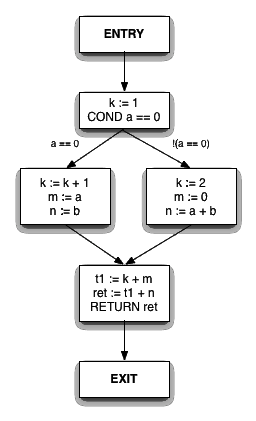
\includegraphics[scale=0.5]{Treehydra-cfg.png}
\end{center}
\caption{Primer grafa kontole toka}
\label{fig:graf}
\end{figure}

Svaki deo koda \ref{ex1} se može predstaviti \emph{grafom kontrole toka (eng. control flow graph, CFG)},
i upravo takva reprezentacija će se koristiti za opis apstraktne interpretacije.
Slika \ref{fig:graf} prikazuje funkciju predstavljenu na ovaj način, koju ćemo koristiti za
opis ovog metoda statičke analize.\\
Neke napomene:
\begin{itemize}
\item Veze između čvorova grafa su predstavljene kao grane, pojavljuju se u slučaju
kada imamo naredbe kontrole toka(petlje, uslovni/bezuslovni skokovi itd.).
\item Naredbe imaju najviše jednu dodelu i tačno jednu operaciju. U slučaju naredbe
sa više operacija, vršimo razdvajanje na naredbe sa po jednom operacijom, čije
ćemo rezultate čuvati u pomoćnim promenljivama.
\end{itemize}

Terminologije:
\begin{itemize}
\item Svaki čvor se zove \textbf{osnovni blok} \emph{(eng. basic block, \textbf{BB})}.
Osnovni blok se definiše tako što ima samo jednu tačku ulaza, i jednu tačku izlaza,
što će reći da nema grananja unutar osnovnih blokova.
\item Naredbe ćemo zvati \emph{instrukcije}, iako one uopšteno mogu imati
različite nazive u zavisnosti od toga koliko operanada primaju.
\item \textbf{Tačka u programu} je zamišljena tačka pre ili posle svake instrukcije.
Funkcija ima dobro definisano stanje u svakoj tački, tako da će se naša analiza
programa uvek referisati na ove tačke.
\end{itemize}


\subsection{Konkretna interpretacija}
\label{subsec:concreteimpr}
Pre nego što prođemo kroz primer koji opisuje proces apstraktne interpretacije,
napravićemo jedan prolaz kroz funkciju koju ispitujemo koristeći konkretne vrednosti
kao ulaz. Pritom ćemo pratiti promenljive unutar funkcije, obraćajući pažnju na
one koje su zadržale istu vrednost tokom izvršavanja. Uzmimo sledeće vrenosti za ulaz
\texttt{a = 0, b = 7}:
\verbatiminput{snippets/ex2_1.txt} 
Dakle, texttt{k = 2} pre nego što se koristi u naredbi \texttt{t1 := k + m}.
Možemo pokrenuti funkciju za ostale ulaze i dobili bismo isti rezultat.
Međutim, ovakav način testiranja nam ne može potvrditi da je \texttt{k = 2} za
sve moguće ulaze. (Doduše može, ali samo ako bismo proverili sve moguće vrednosti
koje promenljiva može da uzme.)


\subsection{Približavanje apstraktnoj interpretaciji}
\label{subsec:approachingabsint}
Obratimo pažnju da za \texttt{k}, u okviru funkcije imamo dve bitne provere:
\texttt{a == 0} i \texttt{a != 0}, dok nam vrednost za \texttt{b} u ovom slučaju
nije bitna. Sada ćemo ispitati vrednost promenljivih u okviru funkcije za dva ulaza:
jedan sa ulazom \texttt{a = 0, b = ?}, a drugi sa ulazom \texttt{a = NN, b = ?},
gde \texttt{NN} označava ne-nula vrednost, dok \texttt{?} označava bilo koju vrednost.
Počnimo sa \texttt{a = 0, b = ?}:
\verbatiminput{snippets/ex2_2.txt}
Primetimo da nam se sada pojavljuju \texttt{NN} i \texttt{?}, apstraktne vrednosti
koje predstavljaju skupove konkretnih vrednosti.
Ostaje još da utvrdimo kako se ponašaju operatori nad apstraktnim vrednostima.
Na primer, u poslednjem koraku, \texttt{ret := t1 + n} postaje \texttt{ret := 2 + ?}.
Kako bismo saznali šta ovo znači, posmatramo skupove konkretnih vrednosti: Ako \texttt{?}
može biti bilo koja vrednost, onda i \texttt{2 + ?} takođe može uzeti bilo koju vrednost,
tako da \texttt{2 + ? $\longrightarrow$ ?}. Preostali slučaj testira \texttt{a = NN, b = ?}:
\verbatiminput{snippets/ex2_3.txt}
Posle ovog koraka se vidi da su pokriveni svi mogući ulazi, kao i svaki deo koda
funkcije, stoga možemo zaključiti da je \texttt{k = 2} uvek tačno pre nego što
dođemo do naredbe \texttt{t1 := k + m}. \\
Procedura koju smo upravo ispratili daje određen uvid kako bismo krenuli u proces
apstraktne interpretacije, ali nismo generalizovali samu proceduru. Tačno smo
znali koje apstraktne vrednosti da koristimo za test slučajeve, i to smo mogli
samo zato što smo imali kao primer jednostavnu funkciju. Ova metoda neće biti
primenjiva na komplikovane funkcije, i nije automatizovana.\\
Drugi problem je što smo posmatrali svaku granu funkcije posebno. Funckija sa \texttt{k} iskaza može imati i do
\texttt{$2^k$} grana, dok funkcija sa petljama ih može imati i beskonačno, i ovo nam onemogućava da imamo kompletnu
pokrivenost.

\subsection{Apstraktna interpretacija kroz primer}
\label{subsec:absintex}
Pre nego što krenemo u sam proces apstraktne interpretacije, treba da odaberemo
skupove apstraktnih vrednosti. Ponekad ne znamo kako da odaberemo skupove takvih
vrednosti, tako da ćemo sada proći kroz funkciju bez odabira ikakvih vrednosti:
Dakle, pokušajmo sa sledećim ulazom: \texttt{a = ?, b = ?}:
\verbatiminput{snippets/ex2_4.txt}
Pošto nemamo informaciju o tome šta je \texttt{a}, krenućemo put obe grane.
Prvo za potvrdnu granu:
\verbatiminput{snippets/ex2_5.txt}
Potom za negativni slučaj:
\verbatiminput{snippets/ex2_6.txt}
U ovoj tački, dva izvršna toka se spajaju. Mogli bismo da nastavimo da ih testiramo
ponaosob, ali znamo da će to dovesti do eksplozije u uopštenom slučaju, tako da ćemo
izvršiti spajanje stanja. Potrebno nam je jedno stanje koje pokriva obe grane:
\verbatiminput{snippets/ex2_7.txt}
Ovo stanje možemo dobiti tako što ćemo spajati promenljivu po promenljivu. Na primer,
\texttt{k} je 2 u jednom i u drugom stanju, tako da je \texttt{k = 2} u rezultujućem
stanju. Za \texttt{m}, ono može biti bilo šta u prvom stanju, tako da iako je ono 0
u drugom stanju, može uzeti bilo koju vrednost u rezultujućem stanju. Kao rezultat dobijamo:
\verbatiminput{snippets/ex2_8.txt}
Možemo nastaviti izvršavanje u jednom toku:
\verbatiminput{snippets/ex2_9.txt}
Gde dobijamo odgovor koji smo želeli, \texttt{k = 2}. Osnovne ideje su bile:
\begin{itemize}
\item Proći kroz funkciju koristeći apstraktne vrednosti kao ulaz
\item Apstraktna vrednost predstavlja skup konkretnih vrednosti
\item Kod kontrole toka gde imamo grananje, krenimo put obe grane
\item Gde imamo spajanje, spajamo izlaz iz obe grane
\end{itemize}
\cite{MozWiki}

\subsection{Primer upotrebe operatora proširenja}
\label{subsec:widening}

Razmotrimo sada primer \ref{ex3}. Jasno je da naša analiza ne može proći kroz petlju svih 10000 puta, u opštem slučaju mi ni ne možemo znati postoji li izlaz iz date petlje. Zato je potrebno upotrebiti gorepomenuti operator proširenja, u ovom slučaju takav da se desni kraj intervala proširi do beskonačnosti što nam daje fiksnu tačku operacije koja se izvršava unutar petlje. \\ 

\lstinputlisting[language=C, caption=Kod sa petljom, label=ex3, showlines=true]{snippets/ex3.cpp}

Na kraju, dobijena stanja ograničavamo uslovom petlje koji zahteva se $x$ nalazi unutar $(-\infty, 10000)$ na početku petlje a unutar $[10000, +\infty)$ na njenom izlazu. Na tabeli \ref{tab:tabela1} prikazane su vrednosti dobijene u toku apstraktne interpretacije. \footnote{Primer je preuzet iz \cite{boulanger}}


\begin{table}[H]
\begin{center}
\caption{Apstraktne vrednosti promenljive x po linijama koda i koracima apstraktne interpretacije.}
\begin{tabular}{|l|l|l|l|l|l|} \hline
stanje& početak& prvi prolaz & drugi prolaz & proširenje & uslov\\ \hline
$x_1$ & $(-\infty, +\infty)$ & $(-\infty, +\infty)$ & $(-\infty, +\infty)$ & $(-\infty, +\infty)$ & $(-\infty, +\infty)$ \\ 
$x_2$ & $[\:]$ & $[1,1]$ & $[1,1]$ & $[1,1]$ & $[1,1]$ \\
$x_3$ & $[\:]$ & $[1,1]$ & $[1,3]$ & $[1,+\infty)$ & $[1,9999]$ \\
$x_4$ & $[\:]$ & $[3,3]$ & $[3,5]$ & $[3,+\infty)$ & $[3,10001]$ \\
$x_5$ & $[\:]$ & $[\:]$ & $[\:]$ & $[\:]$ & $[10000,10001]$ \\ \hline
\end{tabular}
\label{tab:tabela1}
\end{center}
\end{table}



\newpage
\section{Formalizacija} 
\label{sec:Formalizacija}
Označimo izvršno stanje programa u datom trenutku, pod čime se podrazumeva vrednost promenljivih kao i mesto u kodu do koga se došlo, odnosno na koje pokazuje programski brojač, sa $v \in V$ gde je $V$ skup svih takvih stanja. Tada možemo primetiti binarnu relaciju prelaska stanja $v_{0} \rightsquigarrow v_{1}$ koja predstavlja da stanje $v_{1}$ može uslediti za stanjem $v_{0}$. \footnote{Ovo poglavlje se primarno oslanja na \cite{salcianu}, gde se mogu naći dokazi tvrdnji koji su ovde izostavljeni radi sažetosti.} \\

Bitno je napomenuti da se ova relacija ne može zameniti funkcijom koja bi slikala jedno stanje u iduće, jer prelazak može zavisiti od okolnosti koje nisu definisane unutar programa, poput učitavanja podataka ili redosleda izvršavanja instrukcija u slučajevima kada program ima više niti, tako da može postojati više različitih stanja u koje jedno stanje prelazi. Posebno su nam zanimljiva stanja $$... \rightsquigarrow v_{n} \rightsquigarrow v_{n}$$ koja odgovaraju zaustavljanjima programa. \\
 
Budući da je u opštem slučaju jedini način da odredimo $v$ da izvršimo sam program, uopštićemo problem uvođenjem pojma prostora svojstava $L$. Njegovi elementi $l \in L$, koje nazivamo apstraktnim stanjima, obuhvataće svojstva koja stanja u koja program dospeva u datom trenutku imaju. Potrebno je naglasiti da dato apstraktno stanje ne predstavlja svojstva jednog konkretnog stanja, već više konkretnih stanja te da pojedinačne promenljive apstraktnih stanja uzimaju vrednosti iz partitivnog domena odnosno skupa podskupova domena promenljivih u konkretnim stanjima.\cite{denotationalsemantics} \\

Nad prostorom svojstava već možemo definisati funkciju $f_{L}:L\rightarrow L$ koja slika apstraktno stanje u ono koje mu sledi.

Pokazaće se korisno definisati dodatnu strukturu nad $L$: \\
\begin{definicija}
Neka je nad $L$ definisana relacija poretka, odnosno relacija $\sqsubseteq$ takva da za sve $a, b, c \in L$ važi
\begin{enumerate}
\item $a \sqsubseteq a$ (Refleksivnost)
\item ako su $a \sqsubseteq b$ i $b \sqsubseteq a$ tada $a = b$ (Antisimetričnost)
\item ako su $a \sqsubseteq b$ i $b \sqsubseteq c$ tada $a \sqsubseteq c$ (Tranzitivnost)
\end{enumerate}
Ukoliko za svaki podskup $L\prime \subseteq L$ postoji najmanja gornja granica $\bigsqcup L^{\prime}$ i najveća donja granica $\bigsqcap L^{\prime}$ tada se $L$ naziva \emph{potpunom mrežom}. \cite{algebra}
\end{definicija} 

\begin{figure}
\begin{center}
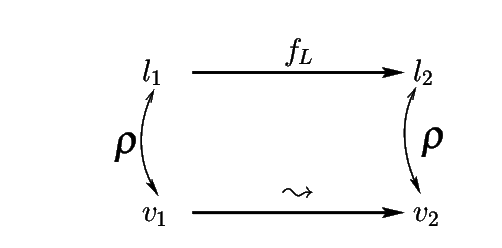
\includegraphics[scale=0.5]{Rho.png}
\end{center}
\caption{Odnos između apstraktnih i konkretnih stanja}
\label{fig:Rho}
\end{figure}

Relacija poretka koju uvodimo nad prostorom svojstava je takva da su veći elementi opštiji od manjih, odnosno da predstavljaju slabije tvrđenje o stanju programa. Tada $\bigsqcup L^{\prime}$ predstavlja disjunkciju apstraktnih stanja u $L^{\prime}$ odnosno stanje u kome važe bilo koja od datih svojstava, dok $\bigsqcap L^{\prime}$ označava stanje u kome sva svojstva važe. Bitne vrednosti su takođe i $\bigsqcup L = \top$ i $\bigsqcap L = \bot$.

Sada želimo dovesti u vezu konkretna stanja programa sa apstraktnim stanjima koja ih modeliraju putem relacije $\rho \subseteq V \times L$ kao što je prikazano na slici \ref{fig:Rho} \footnote{slika je preuzeta sa izmenama iz \cite{salcianu}}. Zahtevamo sledeće od ove relacije:
\begin{enumerate}
\item $\forall v,\, l_{1},\, l_{2},\, (v\: \rho \: l_{1}) \vee (l_{1} \sqsubseteq l_{2}) \Rightarrow (v\: \rho \: l_{2})$
\item $\forall v,\, L^{\prime} \subseteq L, (\forall l \in L^{\prime}, 	(v\: \rho \: l)) \Rightarrow v\: \rho \: (\bigsqcap L^{\prime})$
\end{enumerate}

Ovakvu relaciju nazivamo \emph{relacijom ispravnosti}. Da bi dokazali njenu valjanost u konkretnom slučaju, dovoljno je dokazati je za početno stanje izvršavanja i pokazati da se valjanost čuva pri svakom prelasku u iduće stanje. 


\subsection{Fiksne tačke}
Ukoliko bismo želeli saznati svojstva programa $l$ u nekoj tački izvršavanja, najdirektniji i najprecizniji način bi bio da izračunamo sva apstraktna stanja $l_{i} \in W(l)$ dobijena duž putanja izvršavanja koja vode do te tačke od početnog stanja $l_{0}$ i zatim nađemo $\bigsqcup W(l) = l$. 

Nažalost, u praksi je takav račun nemoguć ili makar veoma zahtevan. Umesto toga, računaju se fiksne tačke funkcije $x = f_{L}(x)$ koje takođe čine potpunu mrežu pod uslovom da je $f_{L}$ \emph{monotona} \cite{tarski}, odnosno da važi $$\forall l_{1},\, l_{2},\, l_{1} \sqsubseteq l_{2} \, \Rightarrow \, f_{L}(l_1) \sqsubseteq f_{L}(l_2)$$ 

 Ako je uz to funkcija i \emph{neprekidna}, $\bigsqcup f_{L}[L^{\prime}] = f_{L}[\bigsqcup L^{\prime}]$, tada se najmanja fiksna tačka može izračunati kao $$\bigsqcup \{ \: f^{n}_{L}(\bot)\: \}_{n \in \mathbb{N}} \quad \text{gde je} \quad f^{0}_{L}(\bot) = \bot \quad \text{i} \quad f^{n}_{L}(\bot) = f_{L}(f^{n-1}_{L}(\bot)) \quad \cite{baranga}$$

Ipak, i ovom slučaju niz $f^{n}_{L} ( \bot )$ može previše sporo konvergirati, zbog čega uvodimo još jedan, grublji, prostor svojstava $M$ koji će služiti kao apstrakcija za $L$. Da bi objasnili odnos između ova dva prostora, moramo uvesti koncept galoaove veze:
\begin{definicija}
Neka su $(A, \geqslant)$ i $(B, \geqslant)$ parcijalno uređeni skupovi a $F : A \rightarrow B$ i $G : B \rightarrow A$ monotone funkcije. Tada je $\langle A, 	F, G, B \rangle$ \emph{galoaova veza} ukoliko važi 
\begin{enumerate}
\item $\forall a \in A, \, a \leqslant G (F (a))$ 
\item $\forall b \in B, \, b \geqslant F (G (b))$
\end{enumerate}
\end{definicija} 

\begin{teorema}
Ako između $L$ i $M$ postoji galoaova veza $\langle L, \alpha, \gamma, B \rangle$ tada je $\rho^{\prime} \subseteq M \times V$, takva da $$m\: \rho^{\prime}\: v \iff \gamma (m)\: \rho \: v$$ takođe relacija ispravnosti.
\end{teorema}

Druga tehnika je korišćenje operatora proširenja $\nabla : L \times L \rightarrow L$ takvog da je $x, y \sqsubseteq x \nabla y$ za sve $x, y$ i pomoću koga se za bilo koji rastući niz $(y_{n})_{n}$ može napraviti niz $$(x^{\prime}_{n})_{n} \quad \text{gde je} \quad x^{\prime}_{0} = y_{0} \quad \text{i} \quad x^{\prime}_{n} = x^{\prime}_{n-1} \nabla y_{n} $$ takav da konvergira u konačnom broju koraka. \\

Najčešće za funkciju prelaska $f_{L}$ pravimo niz $(f^{n}_{\nabla})_{n}$ takav da:
$$
f^{n}_{\nabla} = 
\begin{cases}
\bot,            								  & 	\text{za} \quad n = 0 \\
f^{n-1}_{\nabla} 							      & \text{za} \quad n > 0 \quad \text{i} \quad f_{L}(f^{n-1}_{\nabla}) \sqsubseteq f^{n-1}_{\nabla} \\
f^{n-1}_{\nabla} \nabla f_{L}(f^{n-1}_{\nabla})  & \text{inače}
\end{cases}
$$

Ovime efektivno ubrzavamo nizove koji rastu a zaustavljamo ih u suprotnom, time se sprečava zaglavljivanje prilikom analizi petlji i drugih cikličnih tokova upravljanja. Za limes ovog niza ispostavlja se da je veći od najmanje fiksne tačke, te da je dobro aproksimira. 

\section{Zaključak}
\label{sec:zakljucak}
U ovom radu smo pokušali da predstavimo tehniku apstraktne interpretacije na način koji će biti razumljiv onima koji nisu imali pređašnjeg kontakta sa teorijom verifikacije programa ili semantičke analize. Prišli smo temi iz neformalnog, tehničkog i formalno-matematičkog ugla. Nažalost, ovakva nam podela nije omogućila da zađemo dublje u materiju. Nadamo se ipak da je zahvaljujući njoj čitalac našao u skladu sa svojim sklonostima nešto što bi ga zainteresovalo za dalje proučavanje ove oblasti, jer je apstraktna interpretacija nesumnjivo korisna i visoko prilagodljiva metoda koja pored sadašnjosti ima i svoju budućnost. 


\addcontentsline{toc}{section}{Literatura}
\appendix
\bibliography{Bibliografija} 
\bibliographystyle{plain}

\end{document}
